% !TEX root = ../thesis.tex
% senor characterization
% @author Tobias Wulf
%

\section{Kennfeldmethode zur Charakterisierung von Sensoren}\label{sec:kennfeldmethode-zur-charakterisierung}


Die physikalisch-mathematische Beschreibung von magnetischen Sensormodellen, für eine simulative Nutzung, ist nicht trivial. Jede in \autoref{sec:magnetische-sensoren} zusammengefasste Sensortechnologie birgt bestimmte verhaltensbezogene Eigenschaften in sich. So müssen technologiebasierte Abhängigkeiten in Linearität und Sättigungsverhalten in komplexen mathematischen Gleichungen beschrieben sein. Wobei bestimmte Parameter der Modelle experimentell bestimmt werden müssen \cite{Schuethe2019}. Das stellt einen erheblichen Arbeitsaufwand dar. Der \gls{gl:ags} ist es gelungen diesen Aufwand durch Messmethodik zu umgehen. So ist die \gls{gl:kennfeldmethode} zur Charakterisierung von magnetoresistiven Sensoren entwickelt worden. Das ziel der Messmethode ist es repräsentative Datensätze zu generieren, die physikalische Charakteristiken eines Sensors in sich vereinigen und sein Verhalten zur weiteren Nutzung zugänglich machen.
\newline
Im Labor der \gls{gl:ags} sind automatisierte Messstände für Sensoren verschiedenster Couleur eingerichtet. Je nach Sensortechnologie und Applikation können diese mit unterschiedlichen Messmitteln bestückt werden. So ist es möglich die richtige Stimulanz für die jeweilige Sensorapplikation zu erzeugen. Für das Ausmessen von Winkelsensoren ist ein \gls{gl:kreuzspulenmessstand} zur Anwendung gekommen \cite{Schuethe2019}\cite{Schuethe2020}. Der Messstand eignet sich besonders gut dazu rotierende Magnetfelder zu erzeugen. Was einer idealen Stimulanz für Winkelsensoren entspricht. Das Magnetfeld wird dabei durch ein speziell abgestimmtes \gls{gl:kreuzspulensystem} erzeugt. Die dafür eingespeisten Spulenströme sind dabei direkt proportional zum erzeugten Magnetfeld. Das Anregungsfeld kann somit über Spulenfaktoren zurückgerechnet werden \cite{Schuethe2020}.
\newline
\autoref{fig:magnetfeldstimuluskennfeldmethode} zeigt das verwendete Anregungsfeld zur Charakterisierung. Stimuliert wird in $X$- und $Y$-Richtung, der räumlichen Sensorebene. So verwendet die $H_x$-Feldgenerierung ein dreicksmodulierter Cosinus-Strom. Die $H_y$-Feldgenerierung nutzt ein, mit gleicher Frequenz, dreicksmodulierten Sinus-Strom. Es entstehen dabei steigende und fallende Modulationsflanken bzw. Messverläufe. Es ergeben sich in polarer Darstellung Trajektorien mit wachsender und schrumpfende Amplituden, die durch Rotation einen nach Außen (steigend) bzw. Innen (fallend) gerichteten Verlauf besitzen \cite{Schuethe2019}. Es werden die Spulenströme und Spannungsausgaben des Sensors aufgezeichnet.
\newline
In einem weiteren Evaluierungsschritt sind Stimuli und Sensorsignale programmatisch zu indizieren, um eine gegenseitig Referenzierung zu ermöglichen. Sodass resultierend zweidimensionale \gls{gl:kennfeldpaar}e, bestehend aus je ein \gls{gl:kennfeld} für entsprechende Winkelsensor-Wheatstone-Brücke, als Charakterisierungsergebnis zur Verfügung stehen \cite{Schuethe2019}.


\clearpage


\begin{figure}[tbph]
	\centering
	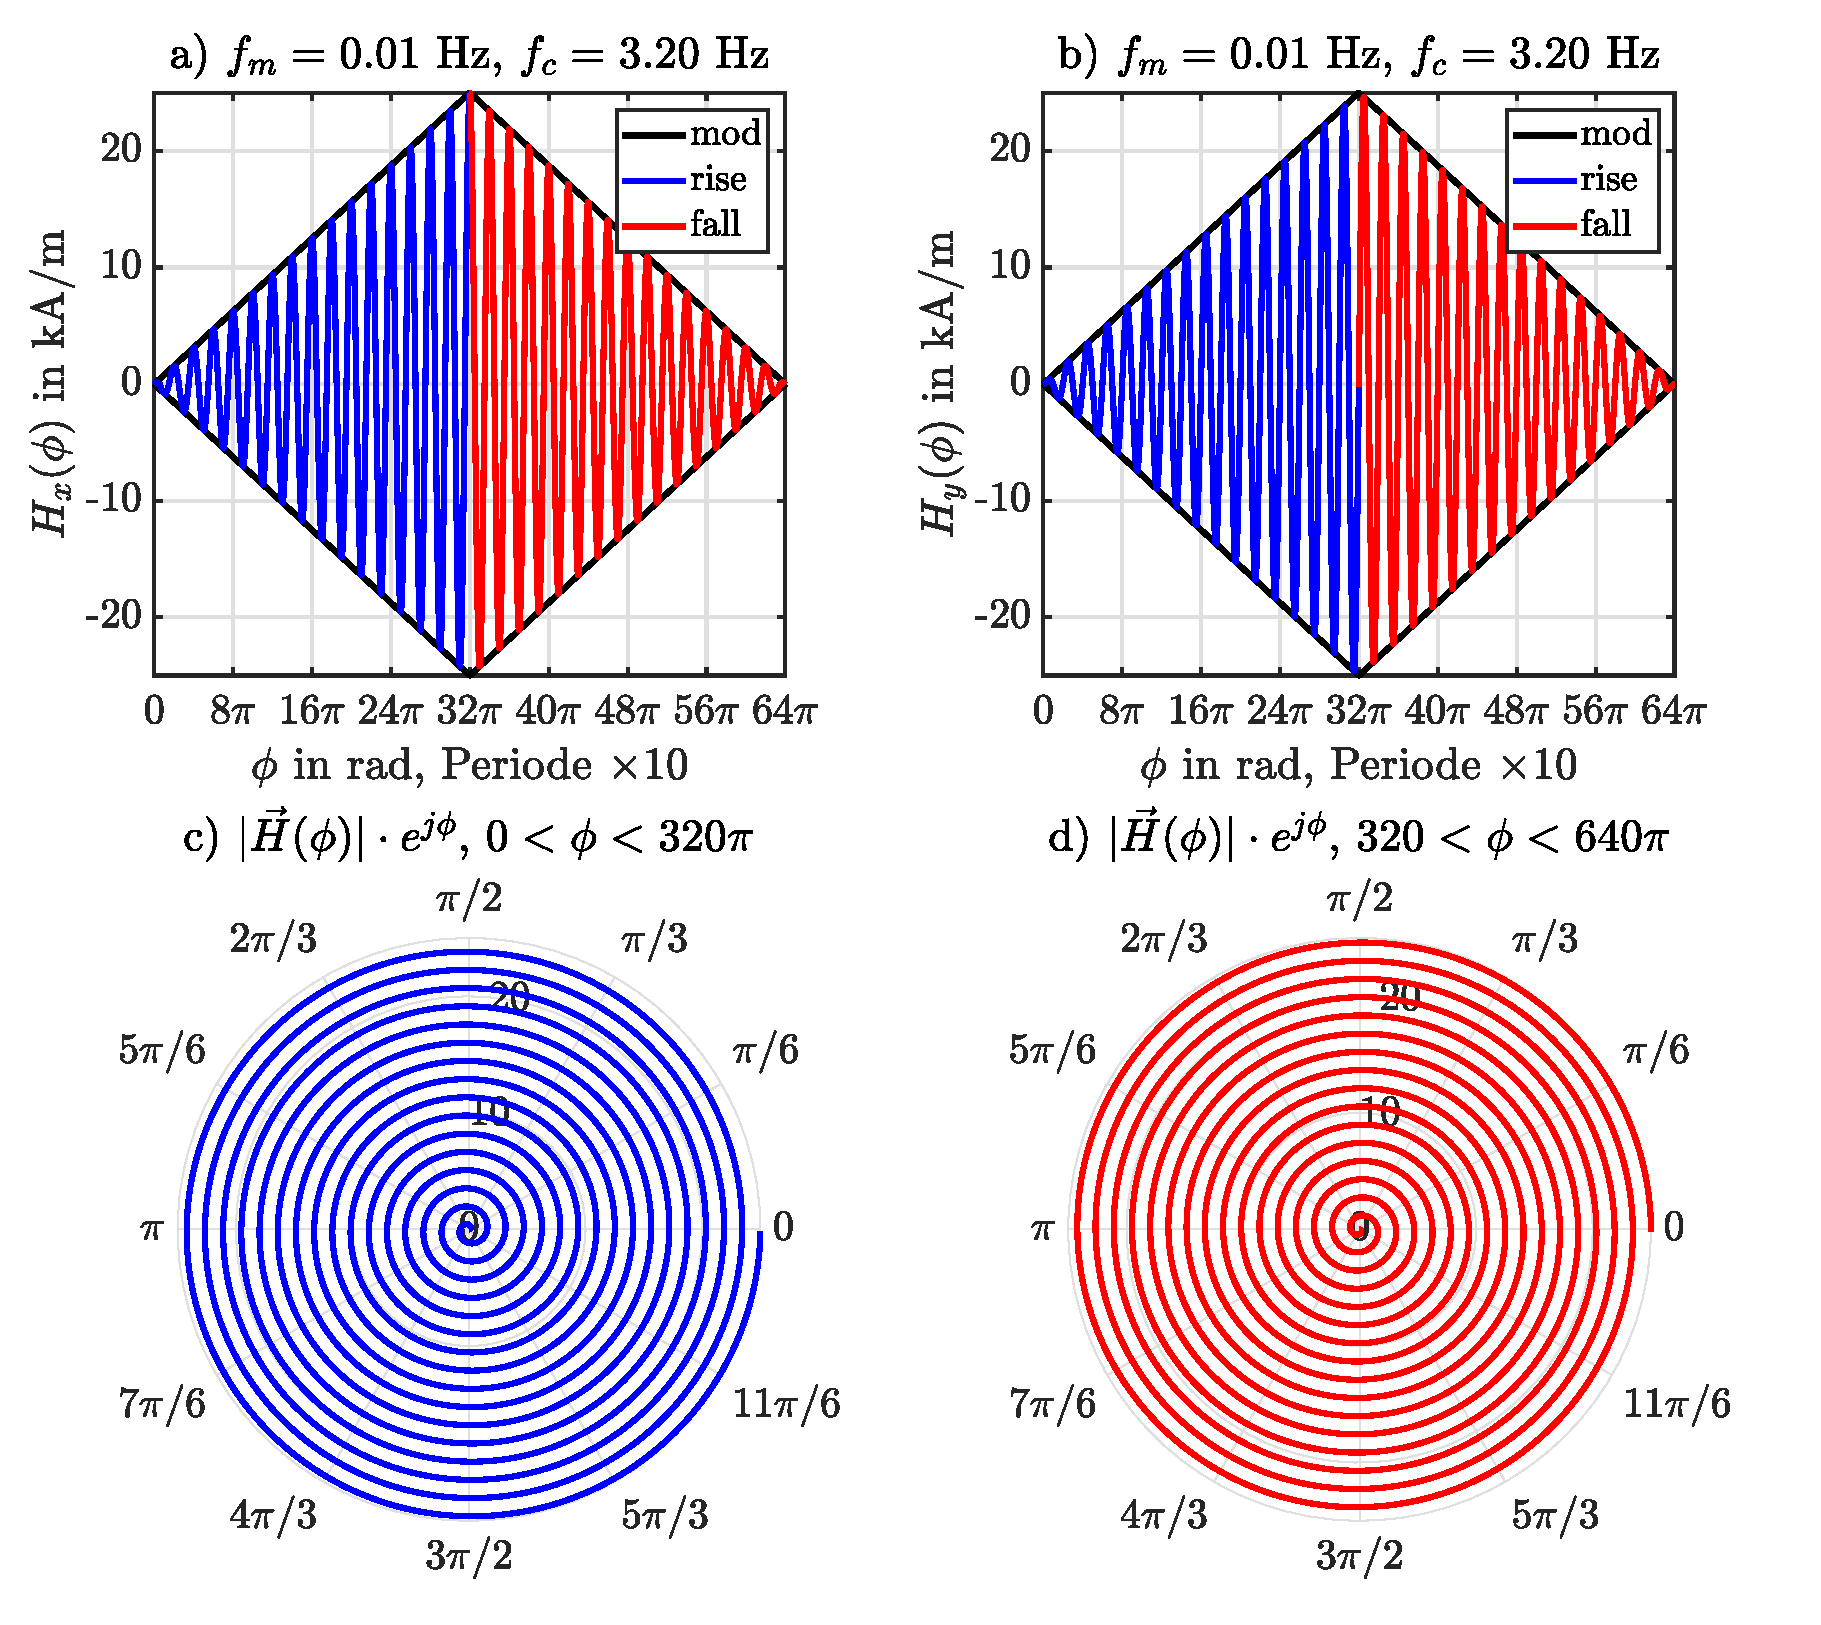
\includegraphics[width=\linewidth]{chapters/images/2-Grundlagen/Magnetfeldstimulus_Kennfeldmethode}
	\caption[Magnetfeldstimulus zur Erzeugung von Sensorkennfeldern]{Magnetfeldstimulus zur Erzeugung von 
		Sensorkennfeldern. Es sind die Bestandteile des magnetischen Sensorstimuli dargestellt, die zum Ausmessen des 
		Sensorkennfeldes in $H_x$- und $H_y$-Richtung verwendet worden sind. Es ist das Prinzip des Verfahrens 
		dargestellt. In a) und b) ist die Dreiecksmodulation des magnetischen Anregungsfeldes abgebildet. Für a) die 
		$H_x$-Feldanregung mit Cosinus-Trägerwelle und für b) die $H_y$-Feldanregung mit Sinus-Trägerwelle. Es sind für 
		beide Anregungsrichtungen niedrige Frequenzen gewählt um ein quasi-statisches Anregungsmagnetfeld zu erzeugen. 
		Es ergeben sich für die Betragsamplitude des Stimulus, in polarer Darstellung c) und d), konzentrische 
		Trajektorien. Diese verlaufen von Innen nach Außen für die steigende Flanke der Amplitudenmodulation c) und von 
		Außen nach Innen für die fallende Flanke d). Die Dreieckmodulationsfrequenz liegt bei $f_m = \SI{0.1}{\hertz}$ 
		und einer Trägerwellenfrequenz $f_c = \SI{3.2}{\hertz}$. Grafik nachempfunden aus \cite{Schuethe2019}.}
	\label{fig:magnetfeldstimuluskennfeldmethode}
\end{figure}


\clearpage


Im \autoref{ch:tdk-datensatz} ist der Kennfelddatensatz eines TMR-Sensors \cite{TDK2016} gezeigt. Der Datensatz dient, als Arbeitsgrundlage für die Sensor-Array-Simulation und ist von der \gls{gl:ags} zur Verfügung gestellt worden. Zur Simulation sind die Kennfelder aus \autoref{fig:TDKuebertragungskennlinien} zu verwenden, a) für die Erzeugung der Cosinus-Funktion und b) für die Sinus-Funktion. Beide Kennfelder zeichnen sich besonders durch ihren linearen Arbeitsbereich zwischen $\pm\SI{8,5}{\kilo\ampere\per\metre}$ aus. Der Arbeitsbereich ist für beide Kennfelder nahezu identisch, zu sehen in c) und als Kreis in a) und b) markiert. 


\vspace{5mm}
\begin{figure}[tbph]
	\centering
	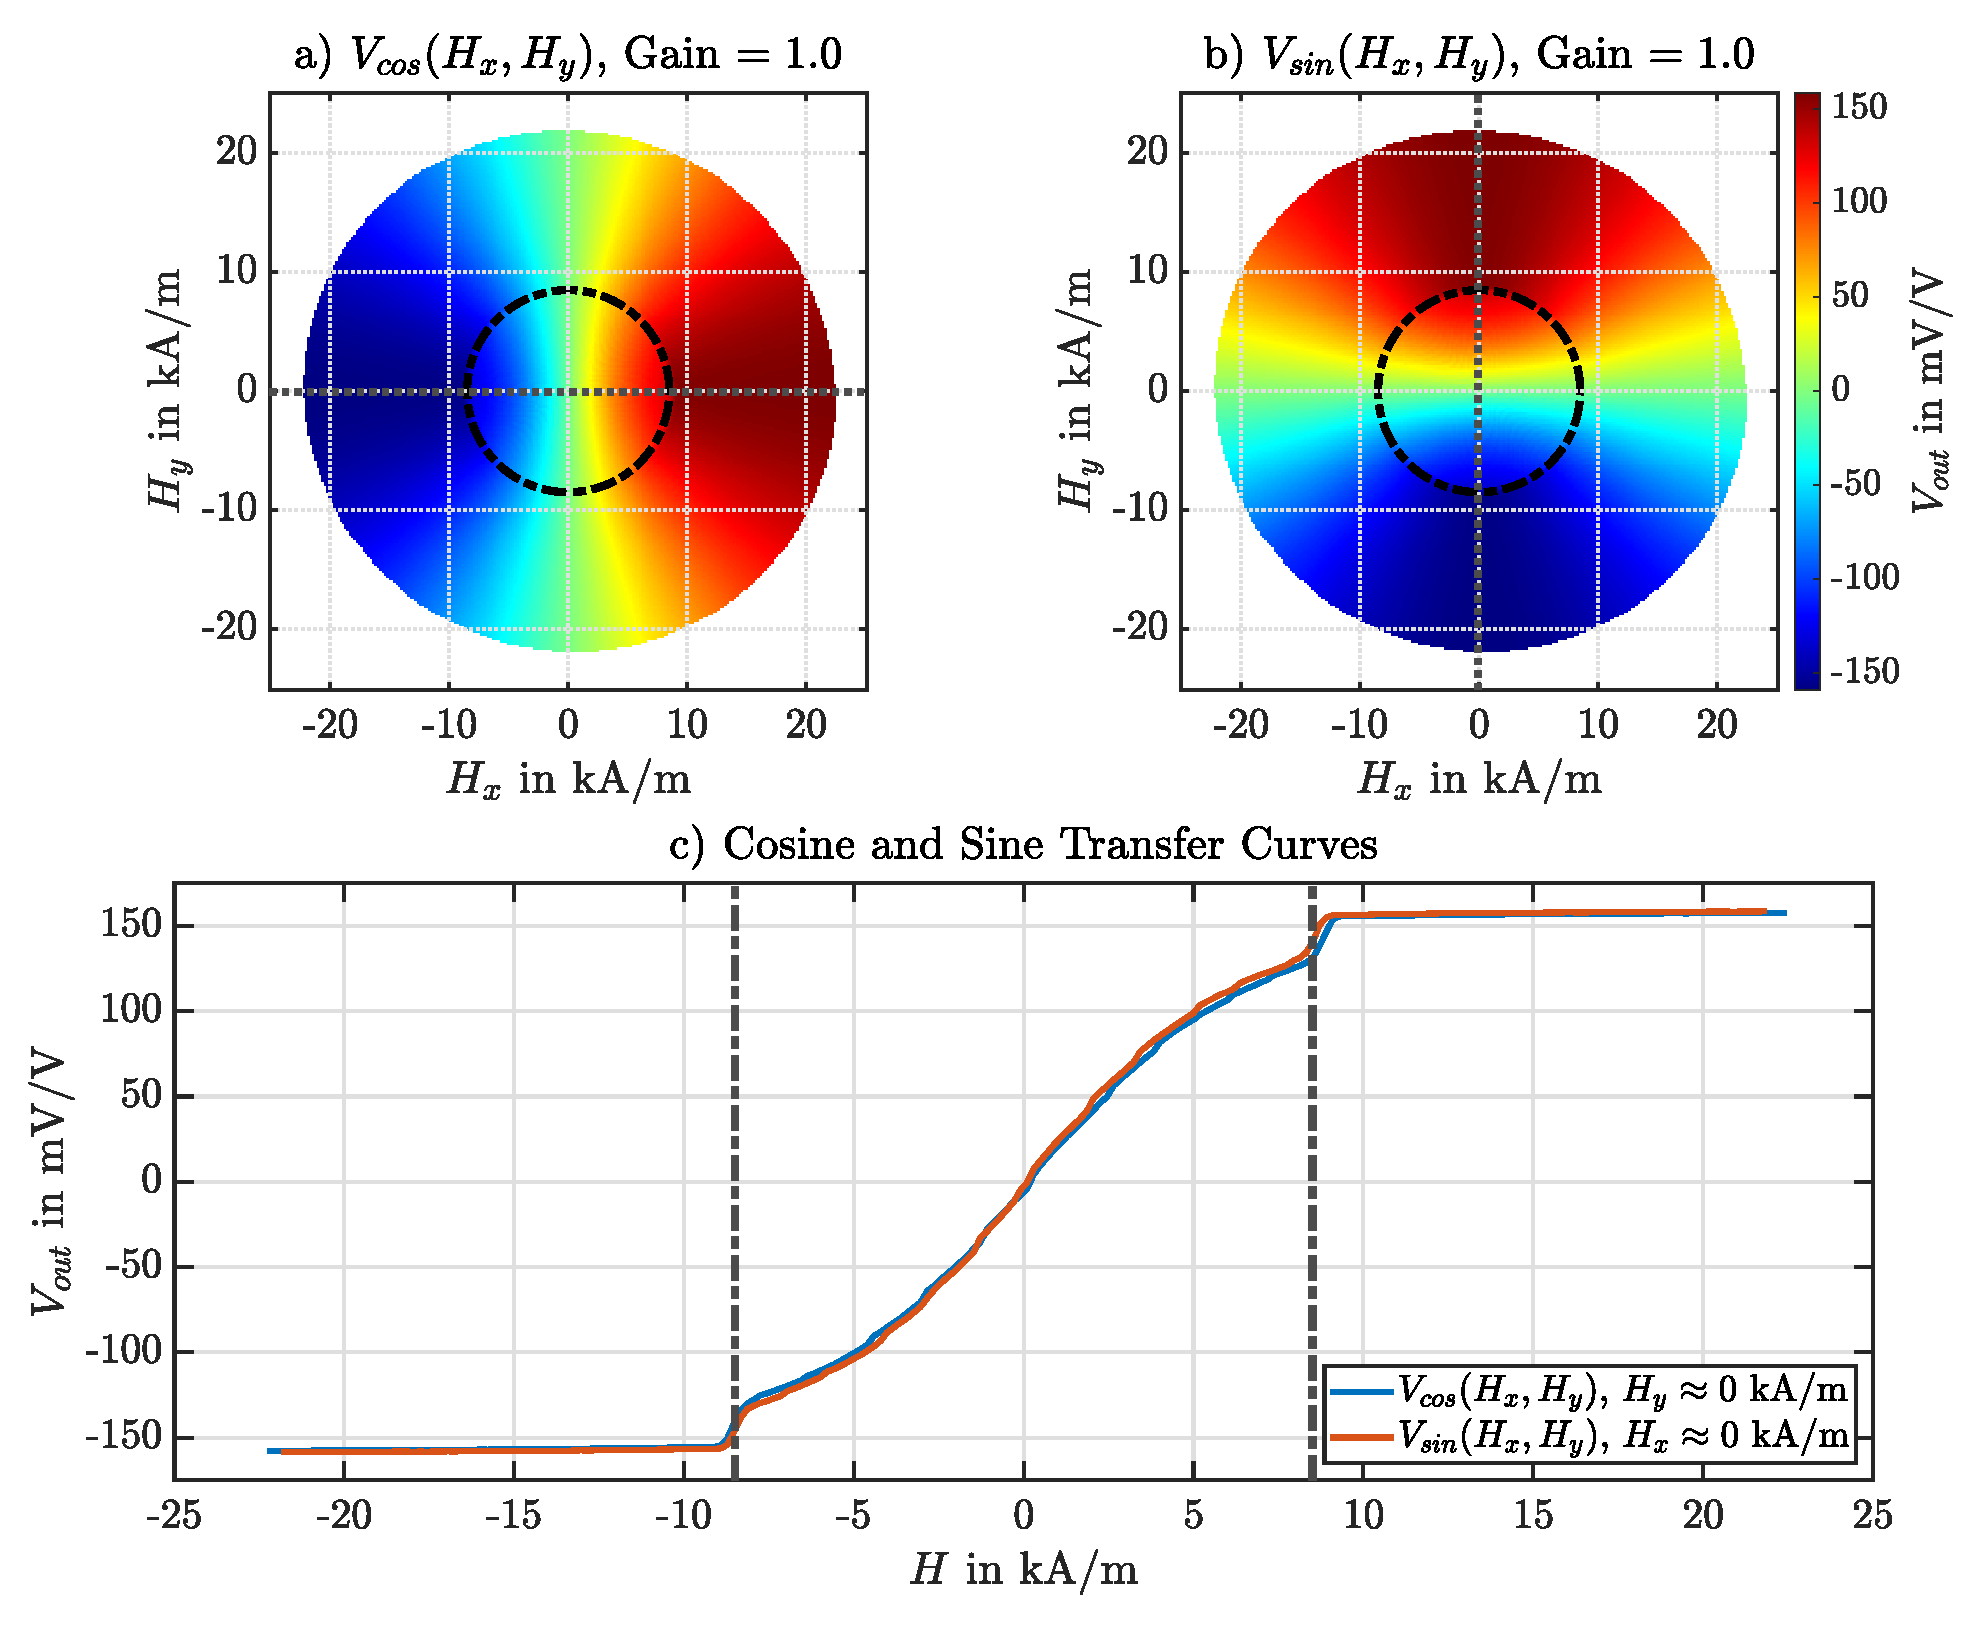
\includegraphics[width=.95\linewidth]{chapters/images/2-Grundlagen/TDK_Uebertragungskennlinien}
	\caption[TDK TAS2141-AAAB Übertragungskennlinie]{TDK TAS2141-AAAB Übertragungskennlinie. Es sind wieder die 
		Kennfelder aus der steigenden Amplitudenmodulation in a) und b). In c) sind die Übertragungskennlinien für den 
		Sensor gezeigt mit Kennzeichnung für den Betrieb auf dem linearen Plateau des Kennfeldes bei 
		$\SI{8.5}{\kilo\ampere\per\metre}$. Ebenfalls zu sehen in a) und b) durch die sich ergebene Kreisbahn mit einem 
		Radius des aufgelegten Intervalls aus c). Grafik nachempfunden aus \cite{Schuethe2019}.}
	\label{fig:TDKuebertragungskennlinien}
\end{figure}


\clearpage


\vspace{5mm}
\begin{figure}[tph]
	\centering
	\includegraphics[width=.7\linewidth]{chapters/images/2-Grundlagen/Approximierter_Kugelmagnet}
	\caption[Approximierter Kugelmagnet]{Approximierter Kugelmagnet. Die Approximation des Kugelmagneten erfolgt 
		über Dipol-Feldgleichung in Näherung des Kugelmagnetfernfeldes. Das Magnetfeld ist auf 
		$\SI{200}{\kilo\ampere\per\metre}$ bei einem Abstand von $\SI{1}{\milli\metre}$ zur Kugelmagnetoberfläche 
		normiert. Der Radius des Kugelmagneten beträgt $\SI{2}{\milli\metre}$.}
	\label{fig:dipolemagnet}
\end{figure}


Auf den TMR-Sensor-Kennfeldern basierende Simulationen, sollten daher so parametriert sein, dass sie innerhalb des markierten Bereiches stattfinden. Zur Generierung von Spannungsausgaben in einer Sensorsimulation, sind für korrespondiere Anregungsfeldstärken entsprechende Referenzwerte aus den Kennfeldern zu entnehmen. Die  Referenzwerte sind normiert und nach \autoref{eq:vout-tdk} in Spannungsausgaben der Wheatstone-Brückenschaltungen umzurechnen. Ein geeignetes Verfahren für die Entnahme von Referenzwerten bietet hier, die in Matlab implementierte $2D$-Interpolation. Diese kann so parametriert werden, dass sie nach dem Nearest-Neighbor-Verfahren für beliebige Feldstärkeneingaben den nächstgelegen Referenzwert ausgibt. Wichtig sind hierbei eine gute magnetische Stimulanz, die den Arbeitsbereich des Kennfeldes trifft.


\clearpage


Als Beispiel für eine passende Anregung soll hier, der in \autoref{fig:dipolemagnet} approximierte, Kugelmagnet dienen. Das Magnetfeld ist so normiert, dass eine Betragsfeldstärke von $\SI{200}{\kilo\ampere\per\metre}$ bei $\SI{1}{mm}$ Abstand zur Magnetenoberfläche anliegt. Die angelegte Skala zeigt, dass ein Sensor mit seinen Kennfeldern aus \autoref{fig:TDKuebertragungskennlinien}, einen Abstand in $Z$-Richtung größer als $\SI{6}{\milli\metre}$ einhalten sollte, um den Arbeitsbereich des Kennfeldes zu treffen. Weitere Beschreibungen und Erläuterungen zur Simulation und Dimensionierung der magnetischen Feldanregung finden sich in beiden folgenden Unterkapiteln \autoref{sec:prinzip-des-sensor-arrays} und \autoref{sec:sensor-array-simulation-dipol-feldgleichung}.



